%----------------------------------------------------------------------------------------
%	PACKAGES AND OTHER DOCUMENT CONFIGURATIONS
%----------------------------------------------------------------------------------------
\documentclass[twoside]{article}
\usepackage{url}
\usepackage{minted}
\newminted{verilog}{mathescape,
               linenos,
               numbersep=5pt,
               gobble=2,
               frame=lines,
               framesep=2mm,
               breaklines=true}
\usepackage{lipsum} % Package to generate dummy text throughout this template
\usepackage{ctex}
\usepackage[sc]{mathpazo} % Use the Palatino font
\usepackage[T1]{fontenc} % Use 8-bit encoding that has 256 glyphs
\linespread{1.3} % Line spacing - Palatino needs more space between lines

\usepackage[hmarginratio=1:1,top=32mm,columnsep=20pt]{geometry} % Document margins
\usepackage[hang, small,labelfont=bf,up,textfont=it,up]{caption} % Custom captions under/above floats in tables or figures
\usepackage{booktabs} % Horizontal rules in tables
\usepackage{float} % Required for tables and figures in the multi-column environment - they need to be placed in specific locations with the [H] (e.g. \begin{table}[H])
\usepackage[colorlinks,
			linkcolor=red,
			anchorcolor=blue,            
			citecolor=green            
			]{hyperref}
\usepackage{lettrine} % The lettrine is the first enlarged letter at the beginning of the text
\usepackage{paralist} % Used for the compactitem environment which makes bullet points with less space between them

\usepackage{abstract} % Allows abstract customization
\renewcommand{\abstractnamefont}{\normalfont\bfseries} % Set the "Abstract" text to bold
\renewcommand{\abstracttextfont}{\normalfont\small\itshape} % Set the abstract itself to small italic text
\usepackage[super,square]{natbib} % 修改文献引用样式
\usepackage{titlesec} % Allows customization of titles
\renewcommand\thesection{\Roman{section}} % Roman numerals for the sections
\renewcommand\thesubsection{\Roman{subsection}} % Roman numerals for subsections
\titleformat{\section}[block]{\large\scshape\centering}{\thesection.}{1em}{} % Change the look of the section titles
\titleformat{\subsection}[block]{\large}{\thesubsection.}{1em}{} % Change the look of the section titles
\usepackage{fancyhdr} % Headers and footers
\pagestyle{fancy} % All pages have headers and footers
\fancyhead{} % Blank out the default header
\fancyfoot{} % Blank out the default footer
\fancyhead[C]{计算机组成与设计$\bullet$ 1月 2018 $\bullet$ 课程设计 } % Custom header text
\fancyfoot[RO,LE]{\thepage} % Custom footer text


\def\equationautorefname{式}%
\def\footnoteautorefname{脚注}%
\def\itemautorefname{项}%
\def\figureautorefname{图}%
\def\tableautorefname{表}%
\def\partautorefname{篇}%
\def\appendixautorefname{附录}%
\def\chapterautorefname{章}%
\def\sectionautorefname{节}%
\def\subsectionautorefname{小小节}%
\def\subsubsectionautorefname{subsubsection}%
\def\paragraphautorefname{段落}%
\def\subparagraphautorefname{子段落}%
\def\FancyVerbLineautorefname{行}%
\def\theoremautorefname{定理}%


%----------------------------------------------------------------------------------------
%	TITLE SECTION
%----------------------------------------------------------------------------------------

\title{\vspace{-15mm}\fontsize{24pt}{10pt}\selectfont\textbf{基于Tomasulo算法的\\乱序执行CPU的实现}} % Article title

\author{
\large
\textsc{颜彬 \(\quad\) 王永锋}\\[2mm] % Your name
\textsc{16337269 16337237} \\ [2mm]
\normalsize 中山大学 教务三班  \\ % Your institution
\vspace{-5mm}
}
\date{2017年1月3日}
%----------------------------------------------------------------------------------------

\begin{document}

\maketitle % Insert title

\thispagestyle{fancy} % All pages have headers and footers
%----------------------------------------------------------------------------------------
%	ABSTRACT
%----------------------------------------------------------------------------------------

\begin{abstract}
	本文主要描述了一种基于Tomasolu算法的支持乱序执行的CPU的实现。网络上很少关于该算法的verilog实现,本文创新性地根据该算法的理论,从模块设计,时序设计等不同角度,独立进行分析、设计该算法硬件层面的实现。在最后,本文还对该算法的优点及不足及可能的提高方法做出了进一步的阐述,并为之后该CPU效率的提高从分支预测,前瞻执行等方面做出了适当的预测和展望。

	\textbf{关键词: }\textbf{乱序执行} \textbf{动态调度} \textbf{verilog} \textbf{CPU运行时间}
\end{abstract}

%----------------------------------------------------------------------------------------
%	ARTICLE CONTENTS
%----------------------------------------------------------------------------------------

\section{选题背景}
\lettrine[nindent=0em,lines=3]{T}omasulo算法是一种在乱序执行流水线CPU中使用的,用于对指令的顺序进行动态调度的算法。在流水线处理器中,先后执行的指令往往具有相关性,如上一条指令将一个数字写进寄存器中,下一条指令马上就要用这一个寄存器中存有的值来进行下一步的计算。这样的数据相关会导致流水线处理器中运行的冲突,这个时候可能可以通过旁路解决,但更多的时候,处理器只能够通过插入一个气泡,堵塞处理器的运行,才能够解决这一种数据冲突。由此,我们可以看出,传统顺序执行的流水线处理器,在处理具有极多数据相关的代码的时候,只能以较低的效率进行计算。\\

为了降低数据相关带来的处理器停顿时间,一般有两种处理方式。\cite{book:zcs}
\begin{description}
	\item[静态调度] 静态调度的流水线依靠编译器对代码进行静态调度,以减少相关冲突。此类调度方式,是通过程序在进行编译的时候就把相关的指令拉开距离,来减少可能产生的停顿。由于是在编译期间进行的指令调度,在程序执行阶段,指令的顺序不能够进行改变,“静态”由此而来。
	\item[动态调度]	动态的指令调度是在程序的执行过程中,依靠专门的硬件对指令进行调度。该种调度方式能够处理一些编译时情况不明的相关,还能够让代码的执行效率与产生指令的编译器解构。目前许多现代的处理器都采用了这种技术。
\end{description}

在本文中,我们关注对指令的动态调度的算法实现。首先探讨一下指令动态调度算法的可行性,要实现指令的动态调度,也就是说我们需要做到在运行过程中,由CPU自行判断哪些指令能够提前运行,同时还能够做到保持数据流和控制异常行为。为了实现这个目的,一个典型的算法是记分牌算法,该算法能够做到与前文无关的指令可以尽早进入执行阶段,从而让处理器的停顿时间减少,但此算法并不能真正解决指令中常常存在的反相关和输出相关,反而,还有可能会让原本的伪相关在乱序执行下变为真相关,从而又从另一个角度增加了处理器的停顿时间。

另一类实现动态调度的算法是Tomasulo算法,该算法解决了记分牌算法的缺陷。相比起记分牌算法,Tomasulo算法中有两个重要的突破\cite{wiki:tomasulo}让它不仅能够最大限度的减少真相关带来的处理器停顿时间,同时直接解决了反相关和输出相关。这两种技术是
\begin{itemize}
	\item \textbf{寄存器换名技术} 
	\item \textbf{CDB公共数据总线}
\end{itemize}
在下文\autoref{algo:tomasulo}中,将会详细描述算法的原理及实现。


%------------------------------------------------

\section{主要工作}
本次课程设计,我们主要完成了以下工作
\begin{compactitem}
	\item 对Tomasulo算法,进行模块设计及时序设计,从而使用硬件的方式实现
	\item 将Tomasulo算法的实现,与CPU的设计结合,整合为一个能够做到支持乱序执行的流水线CPU
	\item 编写机器代码样例,测试CPU的可用性
	\item 分析Tomasulo算法优点及不足,并提出可行的改进方案
\end{compactitem}

%------------------------------------------------
\section{技术路线}

\subsection{数据通路图设计}
\begin{figure}[htp]
    \centering
    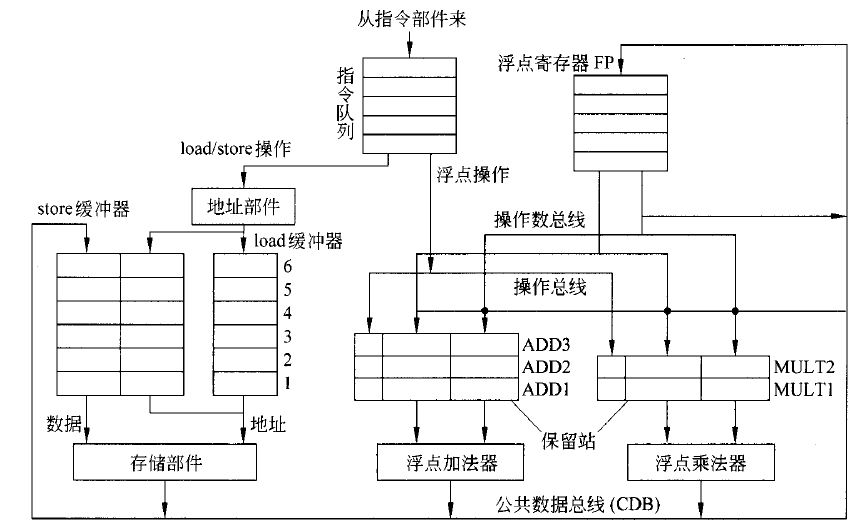
\includegraphics[width=13cm]{"./figure/dataPathDiagram.png"}       
    \caption{乱序执行流水线CPU的数据通路示意图}
    \label{fig:dataPathDiagram}
\end{figure}

\subsection{关键模块设计}
在实现该数据通路的过程中,以下3个关键模块的实现为Tomasulo算法的良好运行打下了良好的基础。
\paragraph{保留站}

% TODO: 保留站端口设计图
\begin{figure}[htp]
    \centering
%	\includegraphics[width=13cm]{"./figure/"}
    \makebox[\textwidth]{\framebox[5cm]{\rule{0pt}{5cm}}}
    \caption{保留站端口设计}
    \label{fig:reservationStation}
\end{figure}

\subparagraph{保留站设计}
\begin{itemize}
    \item 关于保留站的端口设计,可见\autoref{fig:reservationStation}
    \item 当时钟上升沿到达的时候 \\
        1. 由信号isFull反映是否可写及写成功,将对应的值写进保留站中
        (不提供控制写地址的端口,只向外界告知是否写成功)
        2. 从CDB中读取信息,若CDB可用,则上升沿写入对应保留站中的寄存器,并修改相应Qi/Qj
    \item 时钟下降沿到达时,若保留站中存在操作数就绪的指令,则对外输出就绪指令数据及保留站号 \\
        1. 输入信号EXEable若反映ALU不可用, 则对应Busy位不修改,否则将已输出的指令对应的Busy清零
        2. 输出信号OutEn为0反映输出不可用(指令处于未就绪状态),反之则就绪,ALU可写 
\end{itemize}   


\paragraph{公共数据总线CDB}

% TODO:公共数据总线端口设计图
\begin{figure}[htp]
    \centering
%	\includegraphics[width=13cm]{"./figure/"}
    \makebox[\textwidth]{\framebox[5cm]{\rule{0pt}{5cm}}}
    \caption{公共数据总线端口设计图}
    \label{fig:CDB}
\end{figure}

\subparagraph{CDB设计}
CDB中,我们实现了一个优先译码器。当各个器件向CDB发送传播请求时(传送1),只有一个器件能得到接受回应(1),其余器件都得到拒绝回应(0)。通过这种做法,解决CDB总线繁忙的情况,每个时钟周期确保只有一个数据被广播出去。  

\paragraph{寄存器文件}

% & TODO:寄存器文件端口设计图
\begin{figure}[htp]
    \centering
%	\includegraphics[width=13cm]{"./figure/"}
    \makebox[\textwidth]{\framebox[5cm]{\rule{0pt}{5cm}}}
    \caption{寄存器文件端口示意图}
    \label{fig:refFile}
\end{figure}

\subparagraph{寄存器文件设计}
为了能够监视CDB数据总线上的数据,寄存器文件里的每一个寄存器都与CDB直接相连,并在每个时钟上升沿时根据数据总线的信号决定是否更新该寄存器。


\subsection{算法原理}
\label{algo:tomasulo}

% TODO:算法流程图
\begin{figure}[htp]
    \centering
%	\includegraphics[width=13cm]{"./figure/"}
    \makebox[\textwidth]{\framebox[5cm]{\rule{0pt}{5cm}}}
    \caption{指令运行流程:更新PC-指令发射-执行-广播写回}
    \label{fig:flowDiagram}
\end{figure}

结合该数据通路图,该算法的实施流程见\autoref{fig:flowDiagram}
\paragraph{更新PC}
在时钟上升沿时,若当前指令所对应的保留站未满,则更新PC,以备下一条指令写入保留站。

\paragraph{指令流入}
在时钟上升沿,若当前指令对应的保留站未满,则当前指令写入保留站中,并将寄存器的状态表更新为当前写入的保留站号。当前指令中已就绪的操作数,直接从寄存器读进来,从而与寄存器文件解耦合。对于操作数未就绪的指令,在保留站中存好该数据的的最新来源(保留站号,从寄存器状态表读取),等待数据写入。

\paragraph{执行阶段}
保留站能够根据保留站中的所有指令的情况,通过组合逻辑电路判断当前是否有指令所有操作数都就绪,一旦就绪,在时钟上升沿时这条指令就会写到ALU中。

ALU在完成计算并且结果已写入寄存器文件和操作数中后,就会将写成功信号返回给保留站,保留站将该条指令的Busy为置为0,清除该条指令。

\paragraph{广播数据}
ALU执行后,将数据发送到公共数据总线上,当公共数据总线返回成功写入信号后,ALU返回空闲状态等待下一次执行,各保留站和寄存器根据公共数据总线的信息决定是否更新自身数值。
(此过程,保留站中一些需要等待操作数写入指令的就会进入就绪状态)


% \subsection{CPU实现指令集}
% 3. CPU支持指令集的简要介绍


\subsection{仿真及测试}

\paragraph{测试样例1}

\begin{verilogcode}
    001000 00000 00010 0000000000000101 //addi r2, r0, 5 // r2 <- 5
    001000 00001 00011 0000000000001000 //addi r3, r1, 8 // r3 <- 8
    101011 00011 00010 0000000000000100 //sw r2, r3(4)
    100011 00011 00111 0000000000000100 //lw r7, r3(4)
    11111111 00000000 00000000 00000000 //halt
\end{verilogcode}

\paragraph{仿真波形图}
% TODO:回宿舍截一下仿真波形图就好
经过检查各时钟周期各模块的控制信号,以及最后寄存器的结果,验证了该CPU在此样例的正确性。

其他测试样例由于空间限制,就不在此一一放出了。

%------------------------------------------------

\section{项目亮点}
传统Tomasulo教材资料只给出了算法的软件模拟实现或伪代码实现。具体的硬件实现会遇到许多瓶颈。本项目对其中的一些难点做了突破,体现了一些创新性。
\subsection{体系结构特点}
\textbf{该CPU整体体系结构特点为:框架流水线,局部并行化,部件多周期。}  
\begin{description}
	\item[流水线] 总框架大致可以分\textbf{指令发射},\textbf{执行},\textbf{广播}等三个阶段。各个阶段流水执行。即每个时钟周期(几乎)保证有一条指令被执行,一份数据被广播。
	\item[并行化] 多个ALU并行地执行数据。一旦指令的操作数准备完毕,即可从保留站发射到ALU处。各个ALU的运算独立进行,互不干涉。
	\item[多周期] 部件多周期更符合实际情况,本设计中各个执行单元都有~state~部件用于控制状态。所有执行和存储器件都在各个周期内分步骤完成。
\end{description}

\subsection{阵列乘法器}
在ALU的设计中,乘法器的设计利用阵列乘法器加速定点数乘法。  
采用$32 + 16 +... +1=63$个简易的加法电路,按5层的方式排布成阵列,并行地计算乘法。将乘法的运行时间缩短至5个CPU时钟。

% TODO:乘法器示意图
\begin{figure}[!hbp]
\makebox[\textwidth]{\framebox[5cm]{\rule{0pt}{5cm}}}
\caption{此处应有一个乘法器的示意图}
\label{fig:temp1}
\end{figure}

\subsection{Queue in Hardware}
利用硬件实现队列。注意到并解决了所有的所有的难点。包括 
\begin{enumerate}
	\item \textbf{计算空余位置号   }利用组合电路正确计算队列中的空余位置号
	\item \textbf{分配保留站号   } 每次新指令进队时,正确地分配唯一的保留站号
	\item \textbf{处理广播冲突   }当进队的指令中的保留站号恰好为正在广播的保留站号时,队列能正确地将广播中的数据替换指令的数据,再写进队列里
	\item \textbf{正确判断“伪满”   }若队列已满,但下一个周期到来时队列能发射一条指令,则队列实质上仍可以接受指令,并没有处于真正满的状态。本设计能正确识别“伪满”现象,最大限度保证指令流动。
\end{enumerate} 
  
\subsection{Passing Extreme Testcase} 
通过了所有的边界条件测试样例。  
在算法的实际设计中,受到硬件时序的约束,会产生极其多的边界条件。例如
\begin{enumerate}
	\item \textbf{指令队列流出   }指令队列需要判断当前指令所在的保留站是否满。当满时,指令无法流出。
	\item \textbf{广播与写入   }当前广播的信号,恰好对应着当前写入信号的保留站号。此时器件应能正确捕获广播,避免遗漏。
	\item \textbf{执行单元的状态转换   }当执行单元(例如ALU)将运算执行完毕时,它需要考虑以下几种状况:~CDB~总线是否忙碌,保留站是否仍发来请求。  
	ALU的附属器件~state~模块需要对其进行分析,判断其接下来进入的状态。
	\item \textbf{CDB繁忙   }~CDB~是所有“写”操作的唯一总线。当多个器件同时企图写总线时,将会引发冲突,此时需要一个优先译码器决定哪个执行器件的输出可以被广播。被拒绝广播的器件必须阻塞等待,直到CDB总线接受广播。
\end{enumerate}

\subsection{Good Coding Style}
本项目有着良好的代码风格,以确保代码的可读性和可维护性,以备之后项目的进一步发展。
\begin{description}
	\item[采用宏定义增强可读性]将所有常量写入头文件中,便于管理。所有常数都用宏定义代替,增强可读性。
	\item[generate 语法]当大量产生相同器件,或进行相同的连线时,采用~verilog 2001~标准中加入的~generate~语法,以达到效率、准确地描述硬件的效果。
    \begin{verilogcode}
        generate
            genvar i
            for (i = 0; i < n; i = i + 1) begin: loop
                // codes here
            end
        endgenerate
    \end{verilogcode}
\end{description}

%------------------------------------------------
\section{效果评价}

\subsection{实现效果}
我们通过运行一段指定的汇编指令,比较单周期CPU运行时间,多周期CPU运行时间,还有我们实现的乱序执行流水线的CPU运行时间(该时间由vivado仿真得出)。数据可见\autoref{tab:timediff}。由此可见,使用了~Tomasolu~算法实现乱序执行的CPU,在CPU运行效率上有了较大的提高。\\
\paragraph{测试代码}
\begin{verilogcode}
//放测试代码
\end{verilogcode}
% TODO: 补充运行时间对比图
\paragraph{运行结果}
\begin{table}[htp]
    \caption{不同CPU运行时间的对比}
    \centering
    \begin{tabular}{cccc}
        \toprule
        CPU种类 & 单周期CPU & 多周期CPU & 乱序执行流水线CPU \\ 
        时钟周期 & XXX & XXX & XXX \\
        完成一条指令所需周期数 & XXX & XXX & XXX \\
        完成一条指令所需时间 & XXX & XXX & XXX \\
        \midrule
        同一段代码的运行时间 & XXX & XXX & XXX \\
        \bottomrule
    \end{tabular}
    \label{tab:timediff}    
\end{table}

\subsection{不足及反思}
我们对于该算法的实现中,由于时间的限制,并不能将CPU的性能做到最佳,以下是我们发现了该CPU可能存在的一些不足,并思考了相应的解决方案。
\begin{itemize}
    \item ALU数量不足,并行化仍有待提高,在有多条加法语句同时需要执行的时候还可以提高并行化(而且这样的情形存在的概率不低)。因此,我们可以设置多个加法器,多个乘法器,当有多条相同运算的指令同时流入到保留站中时,并且有多条相同运算的指令同时就绪,这些指令就可以在一个时钟周期内并行完成,进而降低了CPU的停顿时间,提高了效率。
    \item 保留站数量的设置并没有达到最佳。保留站的设置数量,关系到能够流入的指令的数量,进而影响到CPU能够并行执行的指令数量,CPU的效率也会受到影响。不难发现,保留站设置得越大,每个周期内保留站内有指令就绪的概率就越高,此时CPU内工作的ALU数量就越大,并行化程度就越高。但从另一方面来看,部件的增加,带来的是硬件的复杂度以及功耗的增加(作为CPU的设计,不仅要考虑仿真时的速度,更重要的是在硬件上运行时的复杂度及功耗),这两者之间的权衡关系,目前以我们的能力还很难把握。
    \item CDB公共数据总线的设计仍可优化。目前的设计是每一个时钟周期CDB接受一个ALU的计算结果并广播出去,这样的设计并非有问题,但效率的降低,源于我们的CDB没有设置结果缓存的区域。试想一下这样的情况,多个ALU同时完成运算,但是此时只能够一个一个广播出去,此时等候的ALU就会处于停顿状态,增加了CPU的停顿时间。要解决这个问题,我们可以在CDB中设置一个硬件队列,这样一来,ALU一旦计算完毕,直接将结果放进CDB中的队列中就自动进行下一次运算,不会再由于无法广播而增加CPU的停顿时间。
\end{itemize}


\section{项目前景}
在现在tomasolu算法资料相当匮乏的情况下,我们仅凭书本还有维基百科上的介绍,先是证明了算法的正确性,然后进行硬件的模块设计,时序设计。

其中硬件的整体架构,参考了书本的结构图,而硬件的接口设计以及时序设计,网上找不到成熟的教程,都是我们从零开始,一步一步摸索实现出来的。
在这个过程中,我们也踩了很多坑,也认识到硬件设计中时序设计的困难。

我们完成的这一个项目,并不是这个CPU设计的结束,而是乱序执行流水线CPU(一个更符合现代处理器架构的CPU)实现的起点,我们需要进一步完善模块的接口设计,我们也还有很多工作需要做(todo list), 我希望,这一个有着详尽文档的设计项目,能够给之后的同学启发,在此基础上,实现分支预测,实现前瞻执行等特性。

\section{鸣谢}
这个项目的完成,需要感谢李国桢老师对我们的大力支持与鼓励,您给了我们很多的学习资料,我们在这些学习资料里收获到了很多实现这个项目必备的知识。

感谢何朝东老师在“计算机组成与设计实验课”课程中的教学,何老师在课堂上讲解了很多与verilog语言有关的知识,同时还详细的说明了vivado软件的用法,让我们受益匪浅。

同时,还需要感谢张晨曦老师及其所著的《计算机体系结构》,该本教材知识点覆盖面广,同时知识讲解透彻,其配套的教学软件更是加深了我们对该算法的理解,这是我们的项目能够成功的前提。

再次感谢给我们支持与鼓励的大家!


%----------------------------------------------------------------------------------------
%	REFERENCE LIST
%----------------------------------------------------------------------------------------
\bibliographystyle{unsrt}
\bibliography{document}
%----------------------------------------------------------------------------------------


\end{document}